\chapter{طراحی ربات}

\section{مقدمه}
در این فصل شروع به طراحی ربات می‌کنیم که در وهله اول باید طرح و مدل ربات را انتخاب کنیم یا از ابتدا مدل را بسازیم. با توجه به نمونه‌های پیشین که در فصل قبلی به آن‌ها اشاره شد؛ با الگو گرفتن از مدل‌های موجود، مدل ربات را طراحی و آن را می‌سازیم. 
در ادامه برای طراحی از   نرم‌افزار سالیدورکس 
\unskip\LTRfootnote{SolidWorks}
استفاده می‌کنیم که تمام جزئیات و نکات را می‌توان در آن اعمال کرد و درنهایت هم مدل نهایی را پرینت کرده و ربات را اسمبل می‌کنیم. در این مسیر با هربار پرینت قطعات و اسمبل ربات، تمام نکات و ایرادات آشکار شده و برای تست بعدی آن‌ها را برطرف می‌کنیم.
\section{الگوبرداری و انتخاب مدل}
همانطور که در قسمت بالا به آن اشاره شد؛ به دلیل وجود نمونه‌های مشابه و امکان الگوبرداری از آن‌ها، مدلی از ابتدا طراحی نشده و از مدل نمونه‌های ساخته شده، استفاده کردیم. به اصطلاح، ما مدل آزاد
\unskip\LTRfootnote{Free-Model}
اقدام به طراحی ربات کردیم؛ به این معنا است که دیگر درگیر جزئیات و قیدهای مدل نشدیم به این دلیل که هدف اصلی پروژه موضوعی دیگری می‌باشد. در این مسیر با تعدادی ربات چهارپا روبرو شدیم که با توجه به مشخصات مطلوب یعنی وزن مناسب، در حدی که موتورها قادر به بلند کردن و حرکت دادن ربات باشند، ابعاد مناسب، به شکلی که ربات قابلیت حرکت کردن در تمام محیط‌ها را داشته باشد و تنها محدود به محیط‌های باز و بزرگ نباشد، به دلیل امکان پرینت پلاستیکی از الگوهای با جنس فلزی و آهنی نمی‌توان استفاده کرد و درنهایت با توجه به محدودیت هزینه سعی بر ساده یازی مدل تا حد امکان کردیم. از چندین ربات الگو گرفتیم که همگی دارای چهارپا می‌باشند و هر پا دارای 3 درجه آزادی
\unskip\LTRfootnote{DOF(Degree Of Freedom)}
است تا بتواند با آزادی عمل مناسبی به سمت هدف حرکت کند. الگو اصلی که در شکل \ref{ربات چهارپا} مشاهده می‌شود نزدیکترین نمونه به مشخصات مطلوب ما می‌باشد.
    \begin{figure}[!h]	
	\vspace{0.2cm}
	\centering
	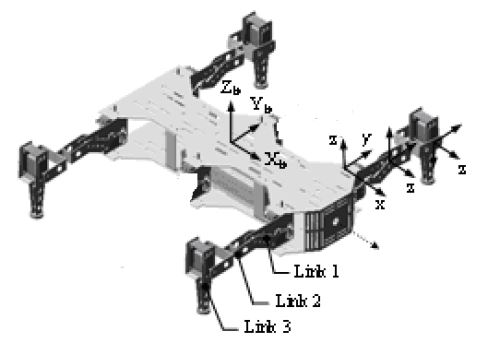
\includegraphics[height=4cm,width=6cm]{./Images/CH2/4_Legged_Robot_1.JPG}
	‌\caption[ربات چهارپا]{ربات چهارپا\cite{Sample}}
	\label{ربات چهارپا}
	\end{figure}

\newpage	
یکی دیگر از نمونه‌هایی که از آن الگو گرفتیم، ربات 
\lr{Titan VIII}
می‌باشد که باز هم دارای چهارپا با سه درجه آزادی می‌باشد اما نحوه جایگیری موتورها با مدل قبلی کمی فرق دارند اما باز هم می‌تواند تمام حرکات لازم را انجام دهد\cite{Titan-VIII}.	
	\begin{figure}[!h]	
	\vspace{0.2cm}
	\centering
	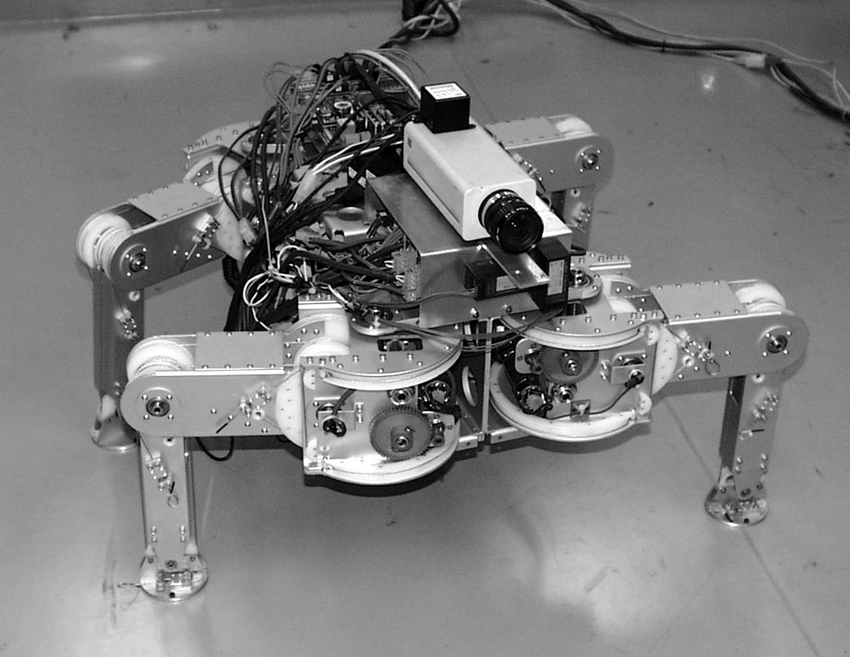
\includegraphics[height=4cm,width=6cm]{./Images/CH2/4_Legged_Robot_TITAN-VIII.png}
	‌\caption[ربات چهارپا\lr{Titan VIII}]{ربات چهارپا\lr{Titan VIII}\cite{Titan-VIII}}
	\label{ربات تایتان}
	\end{figure}
	
\section[نرم‌افزار سالیدورکس]{نرم‌افزار سالیدورکس\cite{SolidWoks}}
سالیدورکس یک نرم‌افزار مهندسی طراحی است که بر روی ویندوز اجرا می‌شود و توسط شرکت فرانسوی داسو سیستمز ارائه و همچنان توسعه داده می‌شود. این نرم‌افزار دارای سه محیط به نام‌های پارت
\unskip\LTRfootnote{Part}
،اسمبلی
\unskip\LTRfootnote{Assembly}
و دراوینگ
\unskip\LTRfootnote{Drawing}
می‌باشد. محیط اول برای رسم قطعه بوده، در محیط دوم قطعات یک مکانیسم بر روی هم سوار شده و در محیط آخر از آن‌ها نقشه مهندسی (معمولاً برای نسخه چاپی) تهیه می‌شود.

سالیدورکس یک مدل‌ساز برای مدلسازی جامدات است که مبتنی بر پارا سالید بوده و از رویکرد پارامتری مبتنی بر ویژگی برای ساخت مدل‌ها و مونتاژها استفاده می‌کند. پارامتر به ثابت‌هایی اطلاق می‌شود که مقدار آن‌ها، شکل یا هندسه مدل یا مونتاژ را تعیین می‌کند. پارامترها هم به صورت پارامترهای عددی نظیر طول خطوط یا قطر دایره بوده و هم به صورت قیدهای هندسی نظیر مماس، موازی، متقارب، هم مرکز و غیره هستند. پارامترهای عددی می‌توانند از طریق استفاده روابط با یکدیگر مرتبط بوده که امکان برآورده ساختن خواسته‌های طراحی را فراهم می‌کند. خواسته‌های طراحی به این معناست که طراح مایل است تا مدل نسبت به تغییرات و به روز آوری‌ها به چه صورت پاسخ دهد. مشخصات
\unskip\LTRfootnote{Features}
به عناصر اصلی سازنده قطعات اطلاق می‌شود. مشخصات اشکال و عملیاتی هستند که قطعه را به وجود می‌آوردند. مشخصات، مبتنی بر شکل نظیر برآمدگی‌ها
\unskip\LTRfootnote{Bosses}
،سوراخ‌ها
\unskip\LTRfootnote{Holes}
و غیره معمولاً با یک نقشه دو بعدی یا سه بعدی آغاز می‌شوند.

نرم‌افزار سالیدورکس دارای ویژگی‌های خاصی می‌باشد که آن را از سایر نرم‌افزارهای 
\lr{CAD}\unskip\LTRfootnote{Computer Aided Design}
مانند کتیا
\unskip\LTRfootnote{CATIA(Computer Aided Three-Dimensional Interactive Application)}
،پرو/اینجینیر
\unskip\LTRfootnote{Pro/ENGINEER}
،یونیگرافیکس
\unskip\LTRfootnote{Unigraphics} 
،مکانیکال دسکتاپ
\unskip\LTRfootnote{Mechanical Desktop} 
و اینونتور
\unskip\LTRfootnote{Inventor} 
شاخص و متمایز می‌نماید:
\begin{itemize}
	\item افزایش سرعت و دقت در طراحی
	\item کاهش خطاها و هزینه‌ها
	\item افزایش قابلیت اطمینان از محصول
	\item امکان طراحی پیچیده و ساختارهای مجتمع
	\item افزایش توانایی در حل مسائل
	\item سرعت بالاتر نسبت به سایر نرم‌افزارها
	\item سهولت کاربری و آموزش در مقایسه با سایر نرم‌افزارهای \lr{CAD}
	\item قابلیت ارتباط با تمامی نرم‌افزارهای ماشین کاری \lr{(edge cam, master cam, power mill…)} و نرم‌افزارهای تحلیل \lr{(Ansys, Adams, Abaqus, Cosmos…)}
	\item قابلیت انجام تحلیل‌های مهندسی با اعمال پارامترها به صورت کاملاً ساده و کاربر پسند.
	\item امکان معادله‌نویسی \lr{(Equation)} بین پارامترها و انداز‌ه‌های مختلف در مدل
\end{itemize}

\section{طراحی و محاسبه ابعاد قطعات}
برای طراحی قطعات به دلیل مدل آزاد بودن، روی طراحی کامل قطعات تمرکز نشد بلکه روی جزئیات آن‌ها و بهتر کردن آن‌ها تمرکز کردیم. در طراحی بسیار مهم است که از چه موتوری استفاده می‌شود تا با توجه به آن، ابعاد قطعات را محاسبه کنیم و مشکلی برای جابه‌جایی هر پا و ربات نداشته باشیم.
با توجه به اینکه سروموتور گشتاور \lr{2.5 Kg/cm} دارد، باید به این موضوع توجه شود که موتور اول هر پا باید بتواند تمام قطعات متصل به پا را یعنی دو موتور و سه لینک پا را جابه‌جا کند.

\newpage
\subsection{نمونه اولیه}
براساس همین مشخصات در ابتدا یک بدنه با ابعاد \lr{140*120*4 mm} طراحی کردیم که شامل دو مستطیل با همین ابعاد است که با چهارتا اسپیسر به هم متصل هستند. برای اینکه وزن موتور اول روی بقیه لینک‌ها ایجاد نشود، روی بدنه بالایی جا برای چهار موتور اول هر پا قرار دادیم که روی بدنه ثابت هستند و با استفاده از دیتاشیت 
\unskip\LTRfootnote{Datasheet}
ابعاد سروموتور را بدست آورده و به اندازه آن روی بدنه خالی می‌کنیم و در آخر هم جا برای پیچ‌های آن قرار میدهیم تا ربات موتور در جای خود ثابت شود و جابه‌جایی آن‌ها وابسته به بدنه است و اگر بدنه از موقعیت کنونی به نقطه‌ای دیگر برود آنگاه چهار موتور هم جابه‌جا میشوند. ملاحظاتی دیگر هم درنظر گرفته شده است مانند فاصله اسپیسرها از بدنه که خیلی نزدیک نباشد، چون اگر این اتفاق بیفتد خیلی شکننده شده و امکان باز شدن اسپیسرها وجود دارد. نکته دیگر هم فاصله بین دوتا موتور می‌باشد که باید به نهوی باشد که لینک اول به راحتی بچرخد و به بدنه ربات برخورد نکند. بدنه پایین هم برای قرارگیری قطعات الکتریکی ربات می‌باشد، به همین دلیل باید فاصله مناسبی بین دو بدنه باشد تا قطعات بدون مشکل قرار بگیرند و همچنین سیم 12تا موتور هم باید به بردی که روی بدنه پایین قرار می‌گیرد متصل شود.

	\begin{figure}[!h]	
	\vspace{0.2cm}
	\centering
	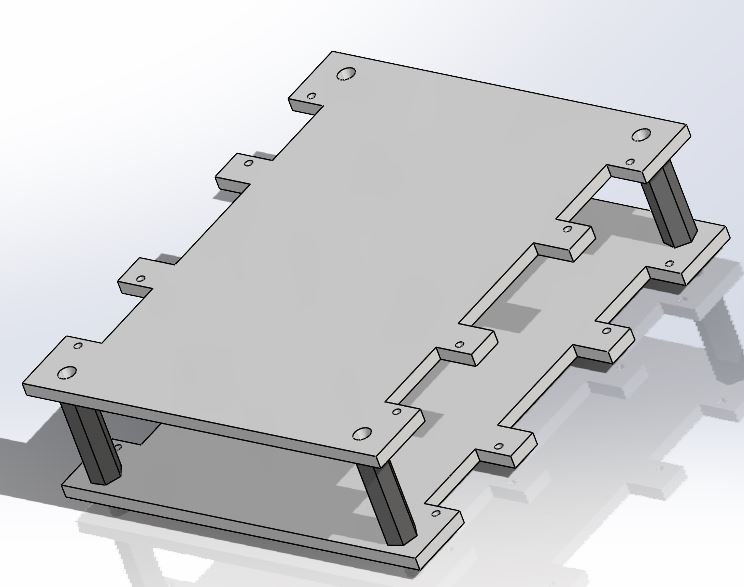
\includegraphics[height=8cm,width=8.5cm]{./Images/CH2/Upper_Bottom_Layer_First.JPG}
	‌\caption{لایه بالایی و پایینی نمونه اولیه}
	\label{بدنه ربات نمونه اولیه}
	\end{figure}

\newpage	
بعد از بدنه به لینک اول می‌رسیم که ابعاد \lr{50*36*8 mm} و تقریبا وزن 3 گرمی دارد که برای سرو موتور هم مشکلی ایجاد نمی‌کند.(برای محاسبه وزن قطعات از نرم‌افزار \lr{Cura} استفاده کردیم که می‌توان جنس موردنظر و بقیه جزئیات را در آن تنظیم کنیم) که مانند بدنه که موتور لینک اول وزنی روی لینک اضافه نمی‌کند، در اینجا هم وزن موتور دوم روی لینک اول قرار می‌گیرد و هیچ تاثیری روی لینک دوم ندارد. نکته بسیار مهمی که وجود دارد این است که روی لینک باید جایی برای قرارگیری شفت درنظر گرفته شود چونکه شفت موتور دندانه‌دار است و نمی‌توان به لینک اتصال داد که درنهایت بتواند لینک را جابه‌جا کند، پس از شفت‌های موجود در کنار موتور استفاده می‌کنیم تا این مشکل برطرف شود. باز هم مانند بدنه باید برای کوتور بعدی هم از لینک اول خالی کنیم تا در آن قرار بگیرد.

	\begin{figure}[!h]	
	\vspace{0.2cm}
	\centering
	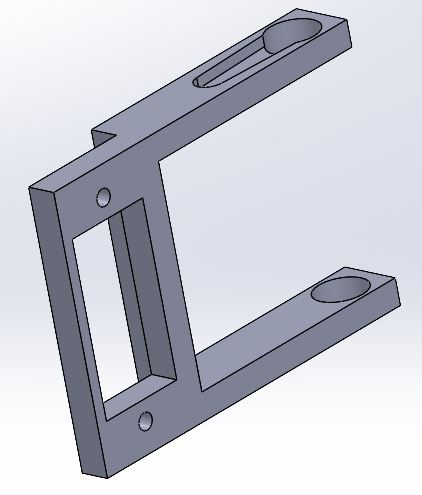
\includegraphics[height=4.5cm,width=4cm]{./Images/CH2/Link1_First.JPG}
	‌\caption{لینک اول نمونه اولیه}
	\label{لینک اول نمونه اولیه}
	\end{figure}
	
لینک بعدی هم مانند لینک قبل است فقط ابعاد و شکل آن متفاوت است. ابعاد این لینک \lr{69*36*8 mm} و وزن 3 گرمی می‌باشد. تفاوت اصلی این لینک با لینک قبلی این است که؛ لینک دوم برای اتصال دو موتور دوم و سوم است و برای همین هم دو جا برای شفت در نظر گرفته شده است. مانند دو \lr{U} است که به هم متصل شده‌اند. محور موتور اول و دوم باهم متفاوت و عمود برهم است. یکی از نکات مهم این لینک ابعاد هر \lr{U} است چونکه وقتی موتور دوم جرکت می‌کند، لینک دوم جابه‌جا می‌شود و نباید ابعاد آن به شکلی باشد که به لینک اول گیر بکند یعنی عمق هر \lr{U} باید از فاصله شفت موتور اول تا انتها لینک اول بیشتر باشد.
%(به دلیل آنکه فاصله شفت موتور اول تا ابتدا لینک از انتها کمتر است پس اگر به انتها لینک برخورد نکند قطعا با ابتدا لینک هم برخوردی نخواهد داشت)

	\begin{figure}[!h]	
	\vspace{0.2cm}
	\centering
	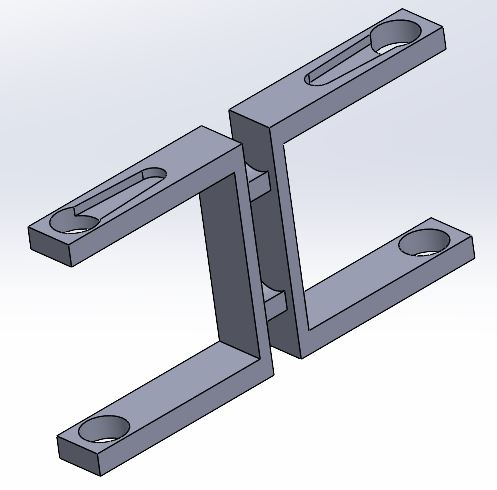
\includegraphics[height=4.5cm,width=4cm]{./Images/CH2/Link2_First.JPG}
	‌\caption{لینک دوم نمونه اولیه}
	\label{لینک دوم نمونه اولیه}
	\end{figure}
	
در نهایت هم لینک آخر(سوم) را داریم که مشخصات آن \lr{71*15*2 mm} و ا گرم است. چون آخرین لینک پا است دیگر نیازی به طراحی فضایی برای قرارگیری شفت نیست و تنها نیاز است فضایی برای پیچ‌های ربات تعبیه شود تا موتور ثابت در جای حود بماند و نلغزد. چالش موجود برای طراحی این قطعه در نقطه تماس آن با زمین است که باید به شکلی باشد که سطح مقطع مناسبی با زمین در تماس باشد چون اگر کمتر باشد باعث می‌شود ربات به درستی نایستد و بلغزد و اگر بیشتر باشد، پاهای ربات اصطحکاک بیشتر از حد معمول خواهند داشت و به سختی جابه‌جا می‌شوند.

	\begin{figure}[!h]	
	\vspace{0.2cm}
	\centering
	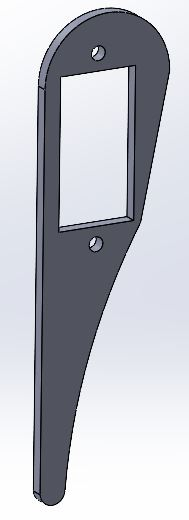
\includegraphics[height=7cm,width=2cm]{./Images/CH2/Link3_First.JPG}
	‌\caption{لینک سوم نمونه اولیه}
	\label{لینک سوم نمونه اولیه}
	\end{figure}
	
	\begin{figure}[!h]	
	\vspace{0.2cm}
	\centering
	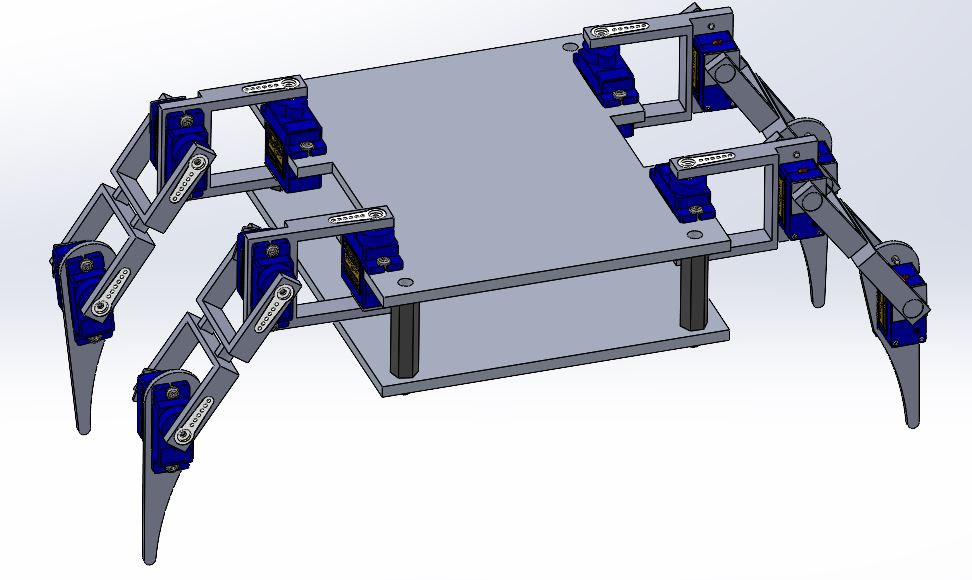
\includegraphics[height=7cm,width=9cm]{./Images/CH2/Robot_First.JPG}
	\caption{نسخه اولیه ربات}
	\label{نسخه اولیه ربات}
	\end{figure}

\subsection{بهبود مدل}
در ابتدا نمونه اولیه قطعات طراحی و پرینت شدند. سپس با بررسی‌های پیاپی مشکلات و ایرادات فطعات پیدا شده و برای بهبود آن‌ها در طراحی تغییراتی ایجاد شدند. 
  
\begin{itemize}
	\item در ابتدا به بدنه ربات می‌پردازیم؛ تقریبا ابعاد بدنه ثابت مانده است اما تغییراتی در آن اعمال شده است مانند قوسی 
	\unskip\LTRfootnote{Curve}
	کردن گوشه‌های تیز بدنه که هم در استحکام و زیبایی آن تاثیرگذار است. دیگر تغییر مهم طراحی یک \lr{U} است برای قرارگیری موتور در آن برای جایگیری دقیق موتور در مکان دلخواه و همچنین نیاز به یک قطعه مانند شفت موتور تا لینک بین این دو شفت ثابت بماند.
	\item و همچنین اگر سیم 12عدد موتور از پایین به برد وصل شود، ممکن است که پاها به آن‌ها برخورد کرده و به درستی کار نکنند پس برای برطرف کردن این مشکل و همچنین کم کردن وزن بدنه، وسط بدنه بالایی را به اندازه‌ای خالی می‌کنیم تا هم سیم‌ها به راحتی و با قابلیت تفکیک عبور کنند هم اینکه قطعه محکم مانده و شکننده نشود.
	
	\begin{figure}[!h]	
	\vspace{0.2cm}
	\centering
	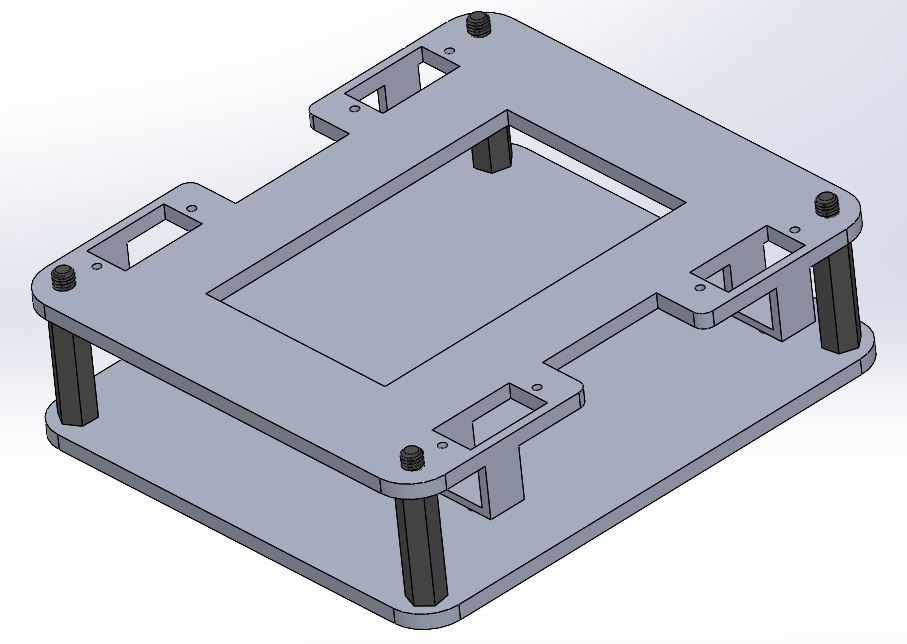
\includegraphics[height=8cm,width=8.5cm]{./Images/CH2/Upper_Bottom_Layer_Final.JPG}
	‌\caption{لایه بالایی و پایینی نمونه نهایی}
	\label{بدنه ربات نمونه نهایی}
	\end{figure}
	
	\newpage
	\item اصلی‌ترین مشکلی که با آن مواجه شدیم، دقیق نبودن پرینتر هست. به عنوان مثال جایی که برای قرارگیری موتورها قرار دادیم کوچکتر از اندازه طراحی شده بود و نیاز بود کمی بزرگتر شود. دو روش برای حل این چالش وجود دارد که ابعاد موتور را خیلی بزرگتر وارد کنیم یا مقدار کمی افزایش دهیم. در حالتی که کمی افزایش دهیم شاید باز هم به راحتی موتور در مکان خود قرار نگیرد اما با کمی فشار یا تراشیدن قطعه بتوان آن را جا زد. اما اگر خیلی افزایش ابعاد را داشته باشیم امکان دارد ربات در مکان خود بلغزد.
	\item لینک اول بسیار نازک‌‌تر از قطعه مدنظر بوده است برای همین ابعاد آن تغییر کرده است. مکانی که شفت در آن قرار می‌گیر بزرگتر شده است به این دلیل که شفت فاصله کمی تا بدنه داشته و امکان آسیب دیدن و شکستن قطعه از آن ناحیه وجود داشته است و همچنین شفت به راحتی در آن قرار نمی‌گرفته و به دلیل فشار موتور کمی از جای خود بیرون زده و گاهی اوقات شفت بیرون از قطعه بوده و نتوانسته لینک را تکان دهد. در نهایت هم ماننده بدنه برای ثبات بهتر موتور روی لینک، موتور را در یک محفظه \lr{U} شکل قرار داده شده است. همچنین فاصله سوراخ پیچ تا بدنه هم افزایش داده شده است تا باز هم اصطحکام بالاتر برود. آخرین نکته در این قطعه که در زیبایی و استقامت آن بسیار حائز اهمیت است، قوسی کردن گوشه‌های تیز موجود در لینک است که وظیفه بسیار مهمی در حفظ سلامت قطعه دارد؛ برای مثال قطعه اولیه اگر از بالا و پایین با دست فشرده شود به راحتی می‌شکند و همچنین قابلیت ارتعاشی دارد که اصلا مطلوب و مناسب نیست.
	
	\begin{figure}[!h]	
	\vspace{0.2cm}
	\centering
	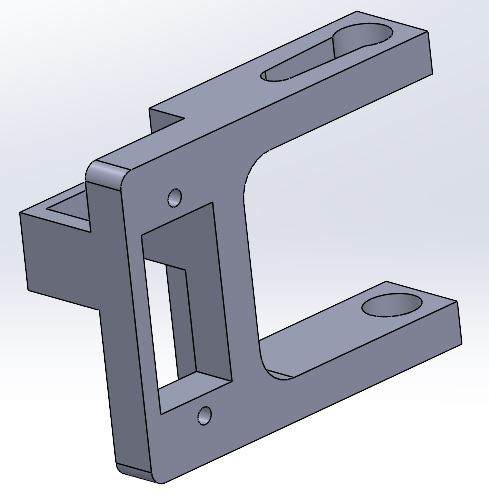
\includegraphics[height=5.5cm,width=5cm]{./Images/CH2/Link1_Final.JPG}
	\caption{لینک اول نمونه نهایی}
	\label{لینک اول نمونه نهایی}
	\end{figure}
	
	\newpage
	\item همانند لینک اول، لینک دوم هم برای جای شفت تغییراتی کرده‌است تا دیگر از جای خود خارج نشده و به درستی عمل کند؛ همچنین گوشه‌های تیز هم قوسی شدند تا در استقامت لینک کمک کنند. سپس تغییری اساسی در آن مشاهده می‌شود که آن هم نحوه اتصال دو \lr{U} می‌باشد که در نمونه اولیه با دو مستطیل کوچک به هم متصل شده‌اند که به شدت شکننده می‌باشد و برای برطرف کردن این مشکل، کل فاصله پر شده‌است و دیگر فضای خالی وجود ندارد. در آخر هم عمق دو تا \lr{U} با هم متفاوت می‌باشد و طرفی که به سمت لینک سوم است کوچکتر از آن طرف قطعه است.
	
	\begin{figure}[!h]	
	\vspace{0.2cm}
	\centering
	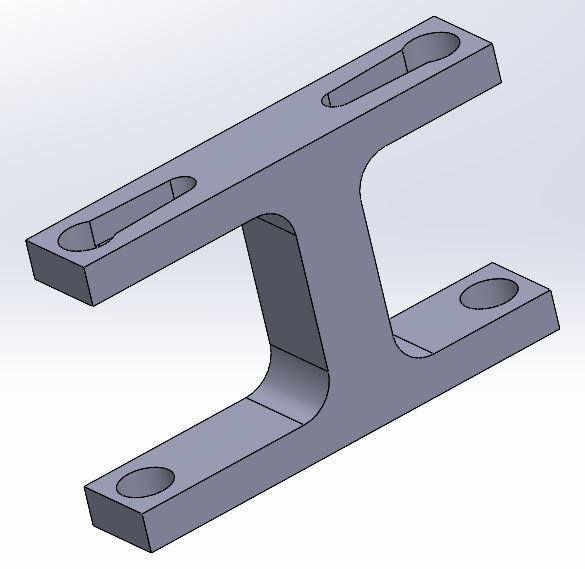
\includegraphics[height=4.5cm,width=4cm]{./Images/CH2/Link2_Final.JPG}
	\caption{لینک دوم نمونه نهایی}
	\label{لینک دوم نمونه نهایی}
	\end{figure}
	
	\item لینک آخر یا همان سوم، کمترین تغییر را نسبت به نمونه اولیه داشته است. ابعاد آن تغییر کرده است تا استحکام بیشتری داشته باشد و همچنین مانند لینک اول قسمتی برای قرارگیری موتور درنظر گرفته شده است.
	
	\begin{figure}[!h]	
	\vspace{0.2cm}
	\centering
	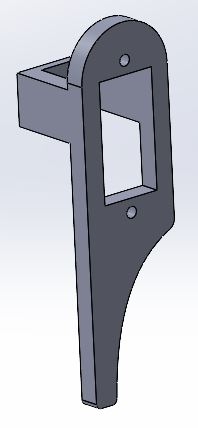
\includegraphics[height=6cm,width=2.5cm]{./Images/CH2/Link3_Final.JPG}
	\caption{لینک سوم نمونه نهایی}
	\label{لینک سوم نمونه نهایی}
	\end{figure}
	
	\begin{figure}[!h]	
	\vspace{0.2cm}
	\centering
	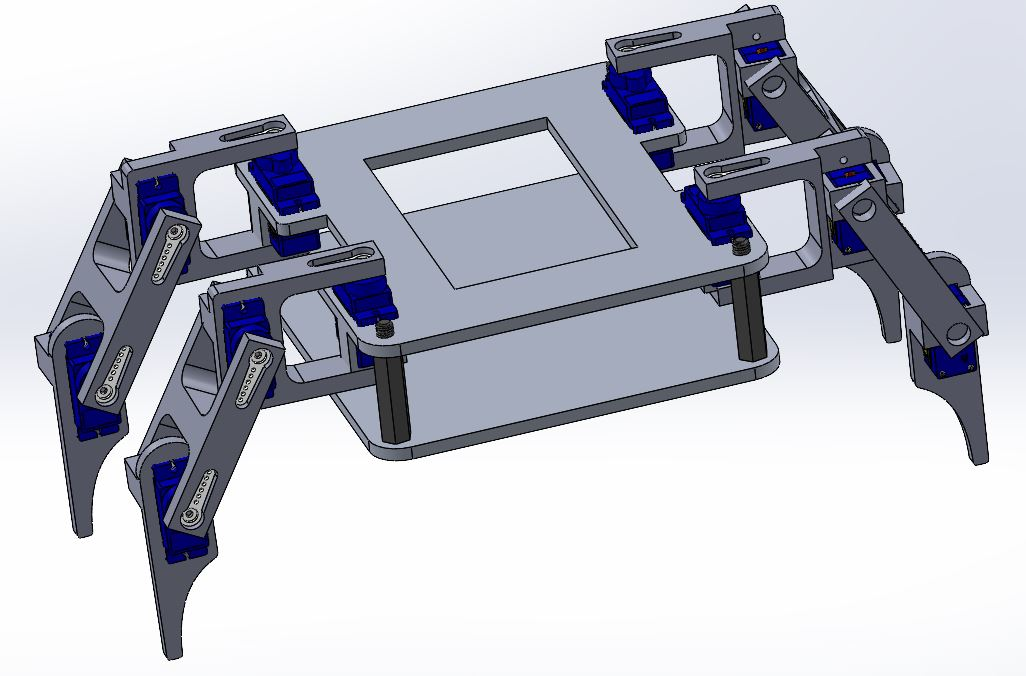
\includegraphics[height=7cm,width=9cm]{./Images/CH2/Robot_Final.JPG}
	\caption{نسخه نهایی ربات}
	\label{نسخه نهایی ربات}
	\end{figure}
	
\end{itemize}

\subsection{نمونه نهایی}
با بررسی‌های فراوان و بهبود مدل در نهایت قطعات پرینت و ربات اسمبل شده است. بدنه ربات با ابعاد \lr{140*120*4 mm}، لینک اول \lr{140*120*4 mm}، لینک دوم \lr{140*120*4 mm} و لینک سوم هم \lr{140*120*4 mm} قطعی شده‌اند. بعد از چندین دفعه پرینت قطعات و تست آن‌ها به نسخه مطلوب و دلخواه رسیدیم که دیگر مشکل شفت، جای موتور، استقامت و ظاهر نامناسب ربات را نداشته باشیم.

	\begin{figure}[!h]	
	\vspace{0.2cm}
	\centering
	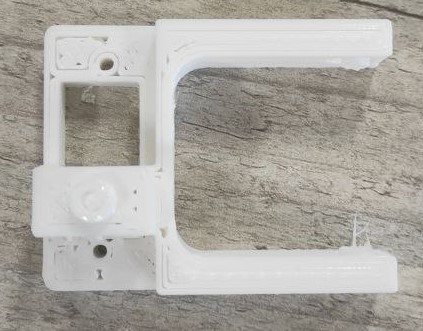
\includegraphics[height=5.5cm,width=5cm]{./Images/CH2/Link1_Printed.jpeg}
	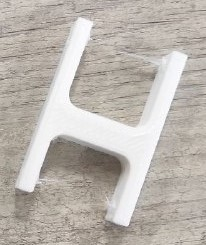
\includegraphics[height=5.5cm,width=5cm]{./Images/CH2/Link2_Printed.jpeg}
	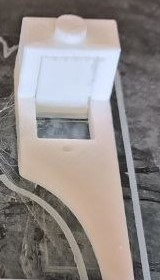
\includegraphics[height=5.5cm,width=2.5cm]{./Images/CH2/Link3_Printed.jpeg}
	\caption{قطعات پرینت شده ربات}
	\label{قطعات پرینت شده ربات}
	\end{figure}
	
\newpage	
\section{جمع بندی}
در کل، در این مسیر طراحی و ساخت ربات، با تمرکز بر جزئیات و بهبود مداوم در اجزاء و مراحل ساخت، به یک نسخه نهایی از ربات دست پیدا کردیم. با تغییر در ابعاد بدنه و لینک‌ها، حل مشکلاتی مانند جابجایی موتورها و تقویت ساختارها، به یک ربات عملی و قابل اعتماد دست یافتیم. این تجربه نشان می‌دهد که با توجه به دقت در تکنیک‌های مهندسی ساده، می‌توان به اهداف خود در ساخت ربات‌ چهارپا دست پیدا کرد؛ که با استفاده از نرم‌افزار سالیدورکس به این مهم دست پیدا کردیم.
	\vspace{1cm}
	\begin{figure}[!h]	
	\vspace{0.2cm}
	\centering
	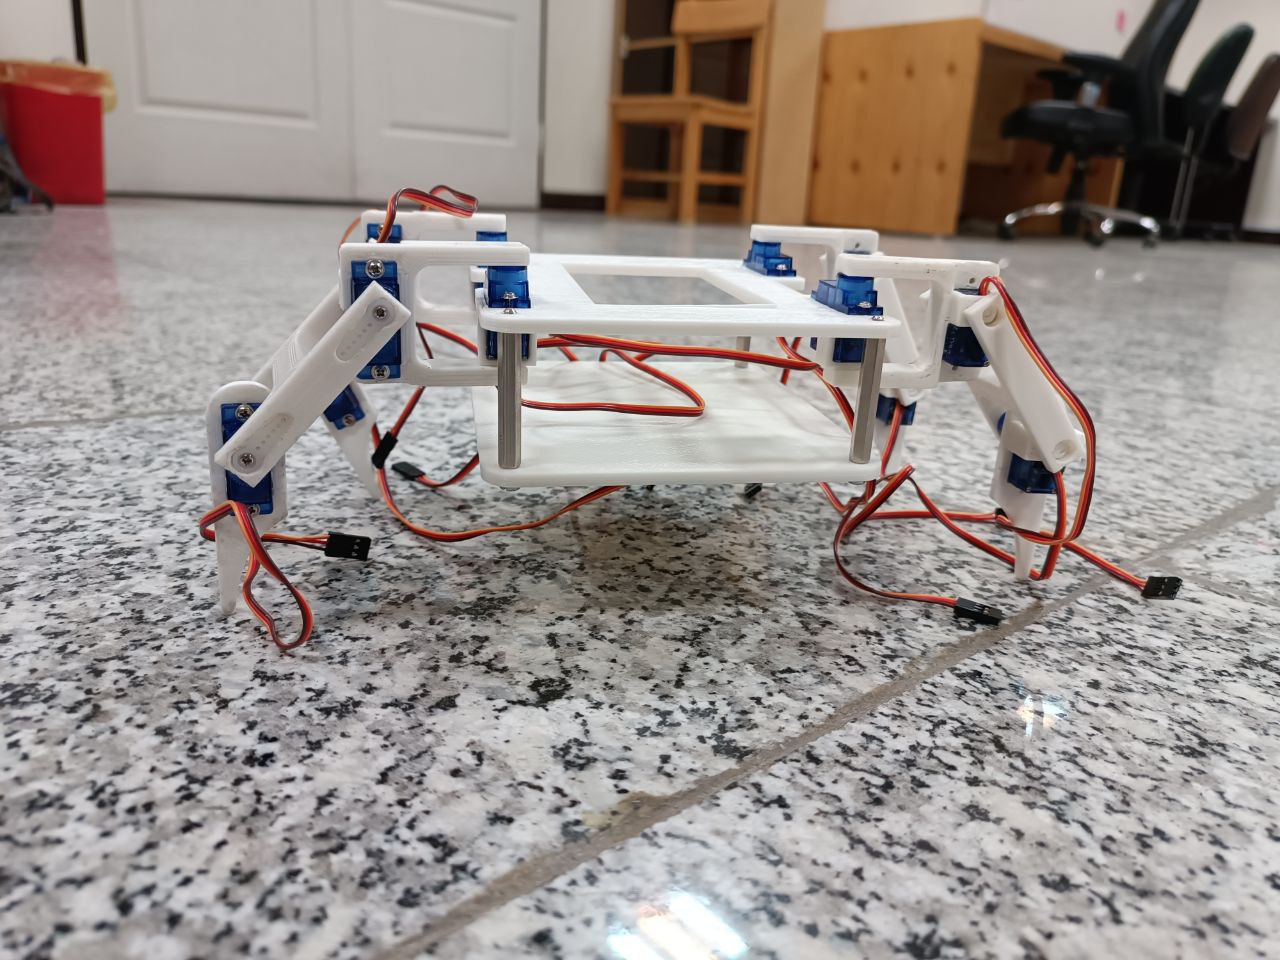
\includegraphics[height=9cm,width=12cm]{./Images/CH2/Assembled_Robot.jpeg}
	\caption{ربات اسمبل شده نهایی}
	\label{ربات اسمبل شده نهایی}
	\end{figure}